\documentclass[border=10pt]{standalone}
\usepackage[T1]{fontenc}
\usepackage{tikz}
\usepackage[svgnames]{xcolor}
\usetikzlibrary{shapes.geometric, arrows.meta, positioning, calc, fit,
                backgrounds, decorations.pathreplacing}

% ---------------------------------------------------------------
% Colour palette (matches solver_flowchart.tex)
% ---------------------------------------------------------------
\colorlet{OrangeFill}{LightSalmon}
\colorlet{OrangeLine}{DarkSalmon!30!Chocolate}
\colorlet{GreenFill}{MediumAquamarine}
\colorlet{GreenLine}{MediumAquamarine!30!Teal}
\colorlet{PurpleFill}{MediumPurple}
\colorlet{PurpleLine}{MediumPurple!30!SlateBlue}
\colorlet{PinkFill}{Thistle}
\colorlet{PinkLine}{Thistle!30!Plum}
\colorlet{BlueFill}{LightSkyBlue}
\colorlet{BlueLine}{SteelBlue}
\colorlet{LimeFill}{YellowGreen}
\colorlet{LimeLine}{YellowGreen!30!Olive}
\colorlet{GrayFill}{LightGray!60!OldLace}
\colorlet{GrayLine}{RosyBrown!50!Silver}

\begin{document}
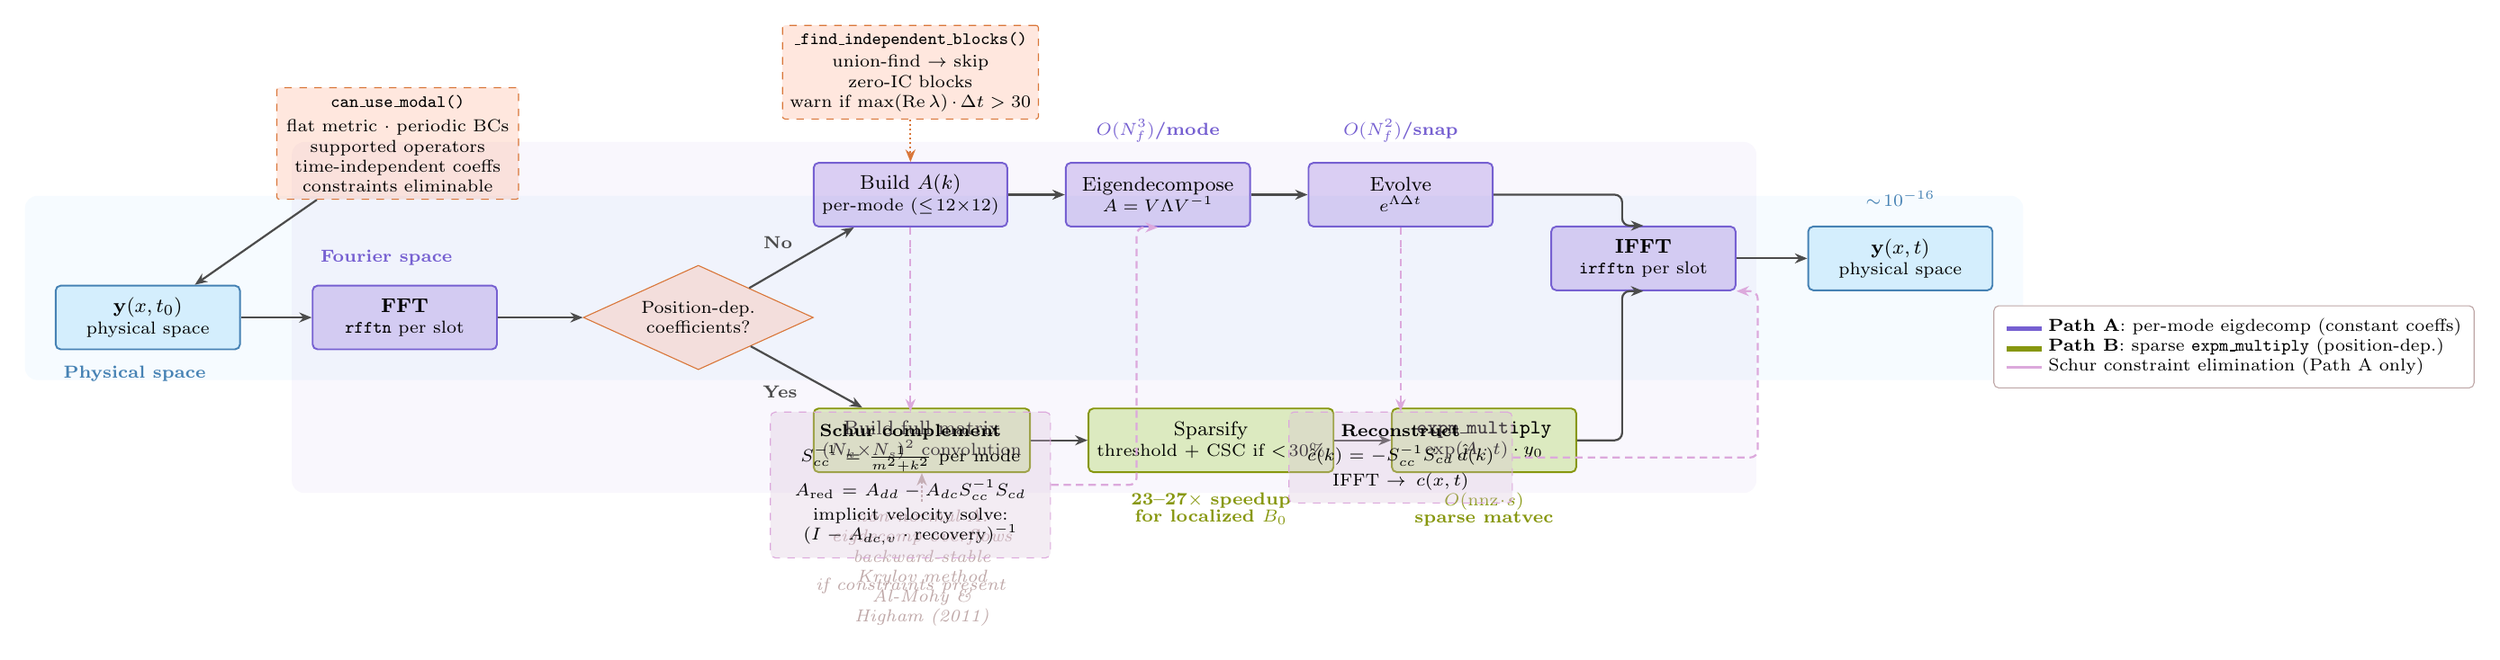
\begin{tikzpicture}[
    % --- Node styles ---
    stage/.style={
        rectangle, rounded corners=2pt, minimum width=2.6cm,
        minimum height=0.9cm, draw=#1, line width=0.7pt,
        font=\footnotesize, align=center, text opacity=1, text=black
    },
    stage/.default={black!70},
    cost/.style={
        font=\scriptsize\bfseries, text=#1, align=center
    },
    cost/.default={GrayLine},
    check/.style={
        rectangle, rounded corners=1pt, draw=OrangeLine, dashed,
        fill=OrangeFill, fill opacity=0.25, font=\scriptsize,
        align=center, text opacity=1, inner sep=3pt
    },
    decide/.style={
        diamond, aspect=2.2, draw=OrangeLine, fill=OrangeFill,
        fill opacity=0.25, font=\scriptsize, align=center,
        text opacity=1, inner sep=2pt, text width=1.8cm
    },
    schur/.style={
        rectangle, rounded corners=2pt, draw=PinkLine, dashed,
        fill=PinkFill, fill opacity=0.3, font=\scriptsize,
        align=center, text opacity=1, inner sep=5pt, text width=3.6cm
    },
    annot/.style={
        font=\scriptsize\itshape, text=GrayLine, align=center
    },
    arr/.style={
        -{Stealth[length=5pt, width=4pt]}, thick, black!70
    },
    yeslbl/.style={font=\scriptsize\bfseries, text=black!70},
    nolbl/.style={font=\scriptsize\bfseries, text=black!70},
    node distance=0.7cm and 1.0cm
]

% ===================================================================
% ELIGIBILITY GATE (top)
% ===================================================================
\node[check, text width=3.2cm] (gate)
    {\textbf{\texttt{can\_use\_modal()}}\\[2pt]
     flat metric $\cdot$ periodic BCs\\
     supported operators\\
     time-independent coeffs\\
     constraints eliminable};

% ===================================================================
% PHYSICAL SPACE INPUT
% ===================================================================
\node[stage=BlueLine, fill=BlueFill, fill opacity=0.3,
      below left=1.2cm and 0.5cm of gate] (input)
    {$\mathbf{y}(x, t_0)$\\[-1pt]\scriptsize physical space};

% ===================================================================
% FFT
% ===================================================================
\node[stage=PurpleLine, fill=PurpleFill, fill opacity=0.3,
      right=1.0cm of input] (fft)
    {\textbf{FFT}\\[-1pt]\scriptsize \texttt{rfftn} per slot};

% ===================================================================
% DECISION: Position-dependent coefficients?
% ===================================================================
\node[decide, right=1.2cm of fft] (branch)
    {Position-dep.\\coefficients?};

% ===================================================================
% PATH A: Per-mode eigendecomposition (upper branch, purple)
% ===================================================================
\node[stage=PurpleLine, fill=PurpleFill, fill opacity=0.3,
      above right=0.9cm and 0.8cm of branch] (matrix_pm)
    {Build $A(k)$\\[-1pt]\scriptsize per-mode ($\leq\!12{\times}12$)};

\node[stage=PurpleLine, fill=PurpleFill, fill opacity=0.3,
      right=0.8cm of matrix_pm] (eigen)
    {Eigendecompose\\[-1pt]\scriptsize $A = V \Lambda V^{-1}$};

\node[stage=PurpleLine, fill=PurpleFill, fill opacity=0.3,
      right=0.8cm of eigen] (evolve_eig)
    {Evolve\\[-1pt]\scriptsize $e^{\Lambda \Delta t}$};

% ===================================================================
% PATH B: expm_multiply (lower branch, lime)
% ===================================================================
\node[stage=LimeLine, fill=LimeFill, fill opacity=0.3,
      below right=0.9cm and 0.8cm of branch] (matrix_full)
    {Build full matrix\\[-1pt]\scriptsize $(N_k {\times} N_s)^2$ convolution};

\node[stage=LimeLine, fill=LimeFill, fill opacity=0.3,
      right=0.8cm of matrix_full] (sparsify)
    {Sparsify\\[-1pt]\scriptsize threshold $+$ CSC if $<\!30\%$};

\node[stage=LimeLine, fill=LimeFill, fill opacity=0.3,
      right=0.8cm of sparsify] (expm)
    {\texttt{expm\_multiply}\\[-1pt]\scriptsize $\exp(A \cdot t) \cdot y_0$};

% ===================================================================
% CONVERGENCE: IFFT + output
% ===================================================================
\node[stage=PurpleLine, fill=PurpleFill, fill opacity=0.3,
      right=0.8cm of evolve_eig, yshift=-0.9cm] (ifft)
    {\textbf{IFFT}\\[-1pt]\scriptsize \texttt{irfftn} per slot};

\node[stage=BlueLine, fill=BlueFill, fill opacity=0.3,
      right=1.0cm of ifft] (output)
    {$\mathbf{y}(x, t)$\\[-1pt]\scriptsize physical space};

% ===================================================================
% ARROWS — main flow
% ===================================================================
\draw[arr] (gate) -- (input);
\draw[arr] (input) -- (fft);
\draw[arr] (fft) -- (branch);

% Path A (upper): No position-dependent → per-mode eigendecomp
\draw[arr] (branch) -- node[yeslbl, above left] {No} (matrix_pm);
\draw[arr] (matrix_pm) -- (eigen);
\draw[arr] (eigen) -- (evolve_eig);
\draw[arr, rounded corners=3pt]
    (evolve_eig.east) -| ([xshift=-0.3cm]ifft.north) -- (ifft.north);

% Path B (lower): Yes position-dependent → sparsify → expm_multiply
\draw[arr] (branch) -- node[nolbl, below left] {Yes} (matrix_full);
\draw[arr] (matrix_full) -- (sparsify);
\draw[arr] (sparsify) -- (expm);
\draw[arr, rounded corners=3pt]
    (expm.east) -| ([xshift=-0.3cm]ifft.south) -- (ifft.south);

% IFFT -> output
\draw[arr] (ifft) -- (output);

% ===================================================================
% COST ANNOTATIONS
% ===================================================================

% Path A costs (above upper branch)
\node[cost=PurpleLine, above=0.15cm of eigen]
    {$O(N_f^3)$/mode};
\node[cost=PurpleLine, above=0.15cm of evolve_eig]
    {$O(N_f^2)$/snap};

% Path B costs (below lower branch)
\node[cost=LimeLine, below=0.15cm of sparsify]
    {23--27$\times$ speedup\\[-1pt]\scriptsize for localized $B_0$};
\node[cost=LimeLine, below=0.15cm of expm]
    {$O(\mathrm{nnz} \!\cdot\! s)$\\[-1pt]\scriptsize sparse matvec};

% Precision (output)
\node[cost=BlueLine, above=0.15cm of output]
    {$\sim\!10^{-16}$};

% ===================================================================
% BLOCK-AWARE CHECK (above per-mode matrix, Path A only)
% ===================================================================
\node[check, above=0.6cm of matrix_pm, text width=3.4cm] (blocks)
    {\texttt{\_find\_independent\_blocks()}\\[1pt]
     union-find $\to$ skip zero-IC blocks\\
     warn if $\max(\mathrm{Re}\,\lambda)\cdot\Delta t > 30$};
\draw[arr, densely dotted, OrangeLine] (blocks) -- (matrix_pm);

% ===================================================================
% PATH B ANNOTATION (non-normal matrix note)
% ===================================================================
\node[annot, below=0.4cm of matrix_full, text width=3.2cm] (posdep_note)
    {non-normal $A$: eigdecomp overflows\\
     backward-stable Krylov method\\
     Al-Mohy \& Higham (2011)};
\draw[arr, densely dotted, GrayLine] (posdep_note) -- (matrix_full);

% ===================================================================
% CONSTRAINT ELIMINATION (Schur complement, Path A only)
% ===================================================================
\node[schur, below=2.6cm of matrix_pm] (schur)
    {\textbf{Schur complement}\\[2pt]
     $S_{cc}^{-1} = \frac{1}{m^2 + k^2}$ per mode\\[2pt]
     $A_{\mathrm{red}} = A_{dd} - A_{dc} S_{cc}^{-1} S_{cd}$\\[2pt]
     implicit velocity solve:\\
     $(I - A_{dc,v}\cdot\mathrm{recovery})^{-1}$};

\node[annot, below=0.15cm of schur] {if constraints present};

% Arrow from matrix_pm down to Schur, then to eigen
\draw[arr, PinkLine, densely dashed, rounded corners=3pt]
    (matrix_pm.south) -- ++(0,-0.4) -| (schur.north);
\draw[arr, PinkLine, densely dashed, rounded corners=3pt]
    (schur.east) -| ([xshift=-0.3cm]eigen.south) -- (eigen.south);

% Recovery arrow from evolve_eig down to reconstruction
\node[schur, below=2.6cm of evolve_eig, text width=2.8cm] (recover)
    {\textbf{Reconstruct}\\[2pt]
     $\hat{c}(k) = -S_{cc}^{-1} S_{cd}\, \hat{d}(k)$\\[2pt]
     IFFT $\to c(x,t)$};
\draw[arr, PinkLine, densely dashed, rounded corners=3pt]
    (evolve_eig.south) -- ++(0,-0.4) -| (recover.north);
\draw[arr, PinkLine, densely dashed, rounded corners=3pt]
    (recover.east) -| ([xshift=0.3cm]ifft.south east) -- (ifft.south east);

% ===================================================================
% BACKGROUND ZONES
% ===================================================================
\begin{scope}[on background layer]
    % Physical space zone (blue tint)
    \node[fit=(input)(output), inner sep=12pt, fill=BlueFill,
          fill opacity=0.08, rounded corners=5pt] {};
    % Fourier space zone (purple tint) — encompasses both branches
    \node[fit=(fft)(ifft)(matrix_pm)(evolve_eig)(matrix_full)(sparsify)(expm),
          inner sep=8pt, fill=PurpleFill,
          fill opacity=0.06, rounded corners=5pt] {};
\end{scope}

% Zone labels
\node[font=\scriptsize\bfseries, text=BlueLine,
      below left=0.1cm and 0cm of input.south west, anchor=north west]
    {Physical space};
\node[font=\scriptsize\bfseries, text=PurpleLine,
      above=0.15cm of fft.north west, anchor=south west]
    {Fourier space};

% ===================================================================
% PATH LEGEND (bottom right)
% ===================================================================
\node[font=\scriptsize, align=left,
      below right=0.2cm and 0cm of output.south east, anchor=north west,
      draw=GrayLine, rounded corners=2pt, inner sep=5pt, fill=white] {
    \textcolor{PurpleLine}{\rule{0.5cm}{2pt}}
        \textbf{Path A}: per-mode eigdecomp (constant coeffs)\\
    \textcolor{LimeLine}{\rule{0.5cm}{2pt}}
        \textbf{Path B}: sparse \texttt{expm\_multiply} (position-dep.)\\
    \textcolor{PinkLine}{\rule[1pt]{0.5cm}{1pt}}
        Schur constraint elimination (Path A only)
};

\end{tikzpicture}
\end{document}
